
\documentclass[12pt,letterpaper]{article}

\usepackage[margin=1in]{geometry}
\usepackage{amsmath,amssymb}
\usepackage{booktabs}
\usepackage{graphicx}
\usepackage{xcolor}
\usepackage{hyperref}
\usepackage{enumitem}
\usepackage{caption}
\usepackage{array}
\usepackage{parskip}
\usepackage{float}
\usepackage{longtable}
\hypersetup{
    colorlinks=true,
    linkcolor=blue,
    urlcolor=blue
}

\begin{document}

\begin{titlepage}
\centering
\vspace*{1.2cm}

{\Large MIE312: Lab 2\par}
\vspace{0.5em}
{\Huge\bfseries Head Losses in Pipes and Fittings\par}
\vspace{1.2em}

{\Large Department of Mechanical and Industrial Engineering\par}
{\Large University of Toronto\par}
\textcolor{white}{\Large Prepared by: Prof. Sullivan} \\
{\Large Fall 2026}
\vfill

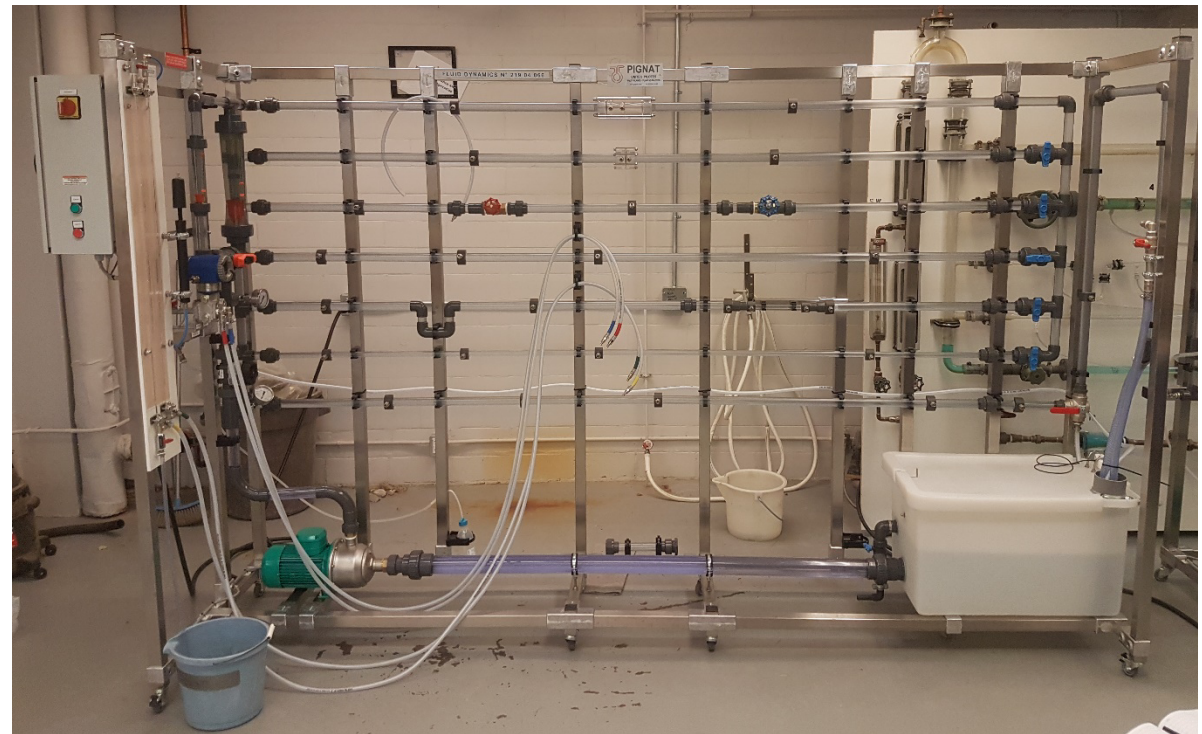
\includegraphics[width=0.78\textwidth]{Lab2_Figures/Cover_image.png}\par

\vfill

\begin{tabular}{|p{0.32\textwidth}|p{0.38\textwidth}|}
\hline
Teaching Assistant: & Eric (Yu Heng) Liang \\ \hline
Email: & \texttt{yh.liang@mail.utoronto.ca} \\ \hline
\end{tabular}

\vfill
\end{titlepage}

\section*{Companion Notebook}

A Google Colab notebook accompanies this lab manual. It automates repeated calculations, generates report-ready plots, and provides a concise summary once raw measurements are entered. The notebook is intended to support the analysis, not replace the required understanding of the equations and physical interpretation.

\begin{center}
\href{https://colab.research.google.com/github/pierresullivan/mie312-labs/blob/main/lab2-pipe-losses/MIE312_Lab2_Head_Losses.ipynb}{\textbf{Open the MIE312 Lab 2 Colab Notebook}}
\end{center}

\subsection*{How to use the notebook}
\begin{enumerate}[leftmargin=*, label=\arabic*.]
    \item Open the notebook link and select \textbf{File $\to$ Save a copy in Drive}.
    \item Run the setup cells to define constants and helper functions.
    \item Enter your measured values in the data-entry tables for Parts 1--4.
    \item Run the remaining cells to compute Reynolds number, identify the flow regime, calculate friction factors using the appropriate model, compare Haaland and Swamee--Jain for turbulent flow, calculate head losses and fitting losses, and generate the Part 4 trendline.
    \item Use the generated tables and plots in your report as needed, but show at least one complete sample calculation and explain the physical meaning of the results.
\end{enumerate}

\noindent\textbf{Important:} The notebook treats \(2100 \le Re \le 4000\) as a transitional range. There is no unique friction-factor correlation prescribed for this regime. Haaland and Swamee--Jain are used as explicit approximations for turbulent flow and may be checked against Colebrook or the Moody chart.

\vspace{1em}
\hrule
\vspace{1em}

\section{Objective}
The objective of this lab experiment is to study head losses in various pipes and fittings and compare experimental and theoretical results.

\section{Experimental Set-Up}
Figure~\ref{fig:apparatus} shows a schematic of the experimental set-up consisting of the following components:
\begin{itemize}[leftmargin=*]
    \item \textbf{Centrifugal Pump:} Transports water at a constant flow rate from the bottom storage tank through the pipes.
    \item \textbf{Storage Tank:} Stores water for the experiment; can be drained and re-filled as needed.
    \item \textbf{Diaphragm Valve:} High-precision adjustable valve to control the total flow rate through the system.
    \item \textbf{Float Flowmeters:} Devices to measure the total flow rate through the system; flowmeter 1 is for low flow rates \((100\text{ to }1000~\mathrm{L/hr})\), while flowmeter 2 is for high flow rates \((600\text{ to }6000~\mathrm{L/hr})\).
    \item \textbf{Pipes (A--G):} Seven clear, horizontal pipes with various fittings and characteristics.
    \item \textbf{Pressure Taps, DPT, and U-tube Manometer:} Used to measure differential pressure and head loss between taps.
    \item \textbf{Venturi, Orifice, Globe Valve, Needle Valve, Sudden Contraction, Sudden Expansion, and Sharp Right-Angle Elbows:} Fittings and irregularities used to study minor losses.
\end{itemize}

\begin{figure}[H]
    \centering
    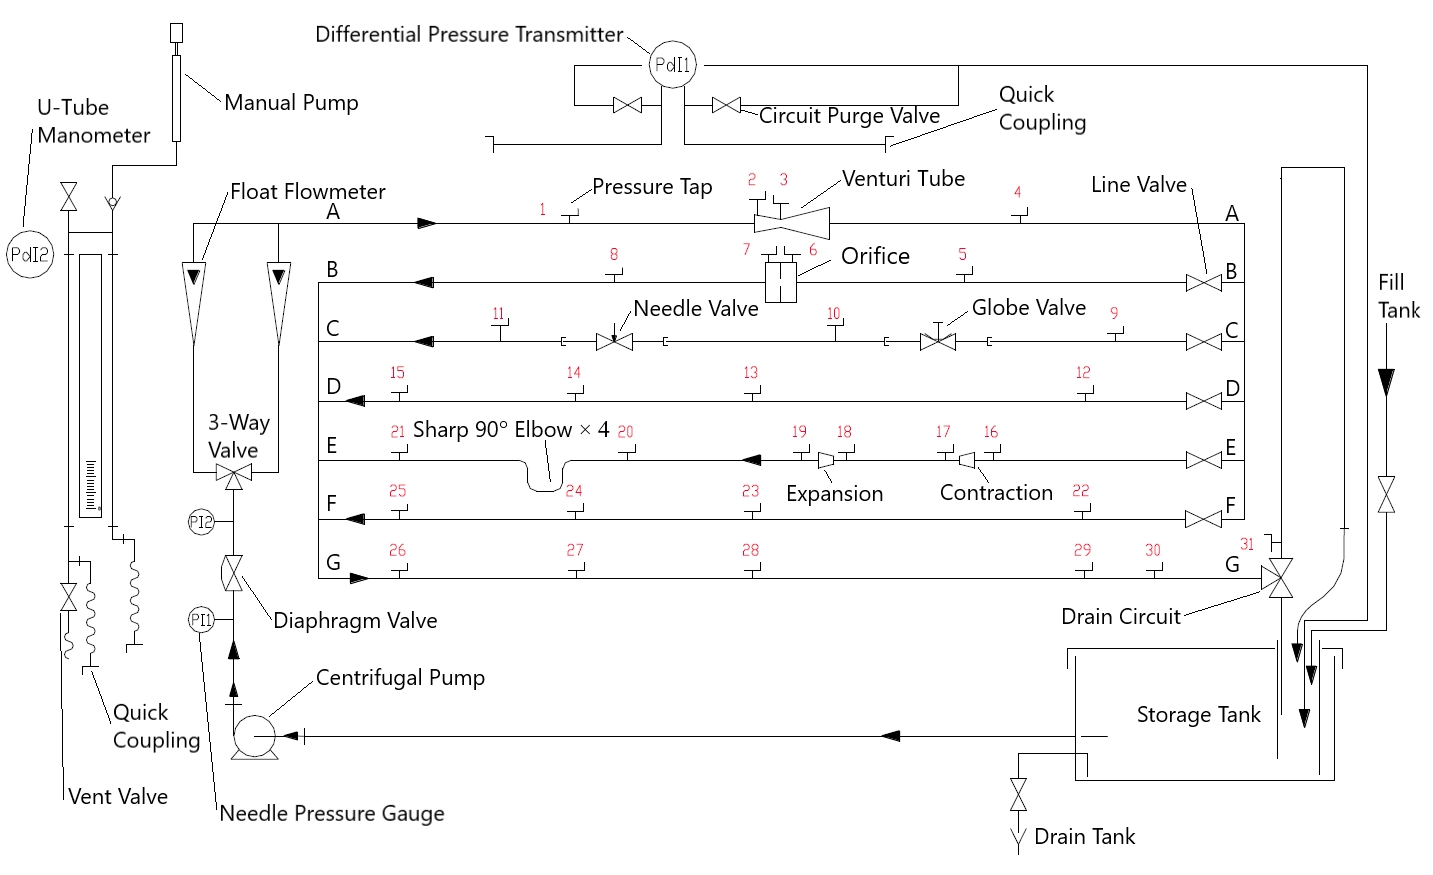
\includegraphics[width=\textwidth]{Lab2_Figures/schematic_original.png}
    \caption{Original apparatus schematic. Pressure taps used in the experiments are identified in Table~\ref{tab:dimensions}.}
    \label{fig:apparatus}
\end{figure}

Some important dimensions are listed in Table~\ref{tab:dimensions}.

\begin{table}[H]
\centering
\caption{Descriptions of pipes and fittings in the experimental apparatus}
\label{tab:dimensions}
\small
\begingroup
\setlength{\tabcolsep}{3pt}
\begin{tabular}{>{\centering\arraybackslash}m{0.06\textwidth} >{\centering\arraybackslash}m{0.08\textwidth} >{\centering\arraybackslash}m{0.10\textwidth} m{0.30\textwidth} >{\centering\arraybackslash}m{0.12\textwidth} m{0.20\textwidth}}
\toprule
Pipe & Flow direction & Pressure tap & Pipe and fitting descriptions & Section lengths, \(L\) (cm) & Inner diameters \(D_i\) (mm) \\
\midrule
A & Right & 1--2 & Straight & 55.5 & \(D_{i,\text{pipe}}=27.2\) \\
A & Right & 2--3 & Venturi inlet -- venturi throat & 3.8 & \(27.2 \rightarrow 15\) \\
A & Right & 3--4 & Venturi throat -- downstream & 60.5 & \(27.2 \rightarrow 15 \rightarrow 27.2\) \\
B & Left & 5--6 & Straight & 52.2 & \(D_{i,\text{pipe}}=27.2\) \\
B & Left & 6--7 & Orifice & 2.6 & \(27.2 \rightarrow 18 \rightarrow 27.2\) \\
B & Left & 7--8 & Straight & 53.2 & \(D_{i,\text{pipe}}=27.2\) \\
C & Left & 9--10 & Globe valve (DN 1") & 98 & \(D_{i,\text{pipe}}=27.2\) \\
C & Left & 10--11 & Needle valve (DN 1") & 98 & \(D_{i,\text{pipe}}=27.2\) \\
D & Left & 12--13 & Rough internal pipe surface & 100 & \(D_{i,\text{pipe}}=27.2\) \\
D & Left & 13--14 & Straight & 50 & \(D_{i,\text{pipe}}=27.2\) \\
D & Left & 14--15 & Straight & 50 & \(D_{i,\text{pipe}}=27.2\) \\
E & Left & 16--17 & Sudden contraction & 8.5 & \(27.2 \rightarrow 13.6\) \\
E & Left & 17--18 & Straight & 20 & \(D_{i,\text{pipe}}=13.6\) \\
E & Left & 18--19 & Sudden expansion & 8.5 & \(13.6 \rightarrow 27.2\) \\
E & Left & 19--20 & Straight & 71.5 & \(D_{i,\text{pipe}}=27.2\) \\
E & Left & 20--21 & Sharp \(90^\circ\) elbow \(\times 4\), \(r=1.5~\mathrm{cm}\) & 95 & \(D_{i,\text{pipe}}=27.2\) \\
F & Left & 22--23 & Straight & 100 & \(D_{i,\text{pipe}}=17\) \\
F & Left & 23--24 & Straight & 50 & \(D_{i,\text{pipe}}=17\) \\
F & Left & 24--25 & Straight & 50 & \(D_{i,\text{pipe}}=17\) \\
G & Right & 26--27 & Straight & 50 & \(D_{i,\text{pipe}}=27.2\) \\
G & Right & 27--28 & Straight & 50 & \(D_{i,\text{pipe}}=27.2\) \\
G & Right & 28--29 & Straight & 100 & \(D_{i,\text{pipe}}=27.2\) \\
G & Right & 29--30 & Straight & 31 & \(D_{i,\text{pipe}}=27.2\) \\
\bottomrule
\end{tabular}
\endgroup
\end{table}

\noindent \textbf{Note:} the absolute surface roughness of the smooth PVC pipes can be taken as \(\varepsilon = 1.5~\mu\mathrm{m}\). The corresponding relative roughness is the dimensionless ratio \(\varepsilon/D\).

\section{Theoretical Background}

\subsection{What is being measured in this lab?}
In this experiment, you are measuring \emph{head loss}, which is the loss of mechanical energy of the flowing fluid between two locations in the system. In pipe flow, head loss is caused by two broad mechanisms:

\begin{itemize}[leftmargin=*]
    \item \textbf{Major losses:} frictional losses distributed along the wall of a straight pipe over a finite length.
    \item \textbf{Minor losses:} local losses caused by fittings or abrupt geometry changes such as valves, elbows, sudden contractions, sudden expansions, venturis, and orifices.
\end{itemize}

The purpose of this lab is to compare measured head losses to theoretical predictions for both of these mechanisms, and to understand how flow rate, roughness, diameter, and fittings affect the result.

\subsection{Laminar, Transitional, and Turbulent Flow}
The first step in most pipe-flow calculations is to identify the flow regime using the Reynolds number:
\begin{equation}
Re = \frac{\rho \bar{V} D}{\mu}
\label{eq:reynolds}
\end{equation}
where:
\begin{itemize}[leftmargin=*]
    \item \(\rho\) is the fluid density \((\mathrm{kg/m^3})\),
    \item \(\bar{V}\) is the mean velocity \((\mathrm{m/s})\),
    \item \(D\) is the internal pipe diameter \((\mathrm{m})\),
    \item \(\mu\) is the dynamic viscosity \((\mathrm{Pa\cdot s})\).
\end{itemize}

For internal pipe flow, the usual classification is:
\begin{center}
\begin{tabular}{cc}
\toprule
Reynolds Number & Flow Regime \\
\midrule
\(Re < 2100\) & Laminar \\
\(2100 < Re < 4000\) & Transitional \\
\(Re > 4000\) & Turbulent \\
\bottomrule
\end{tabular}
\end{center}

This classification appears in the lab material and is specifically for pipe flow. The velocity profile is strongly influenced by the flow regime: laminar flow gives a parabolic profile, while turbulent flow produces a much flatter time-averaged profile with steep gradients near the wall.

\begin{figure}[H]
    \centering
    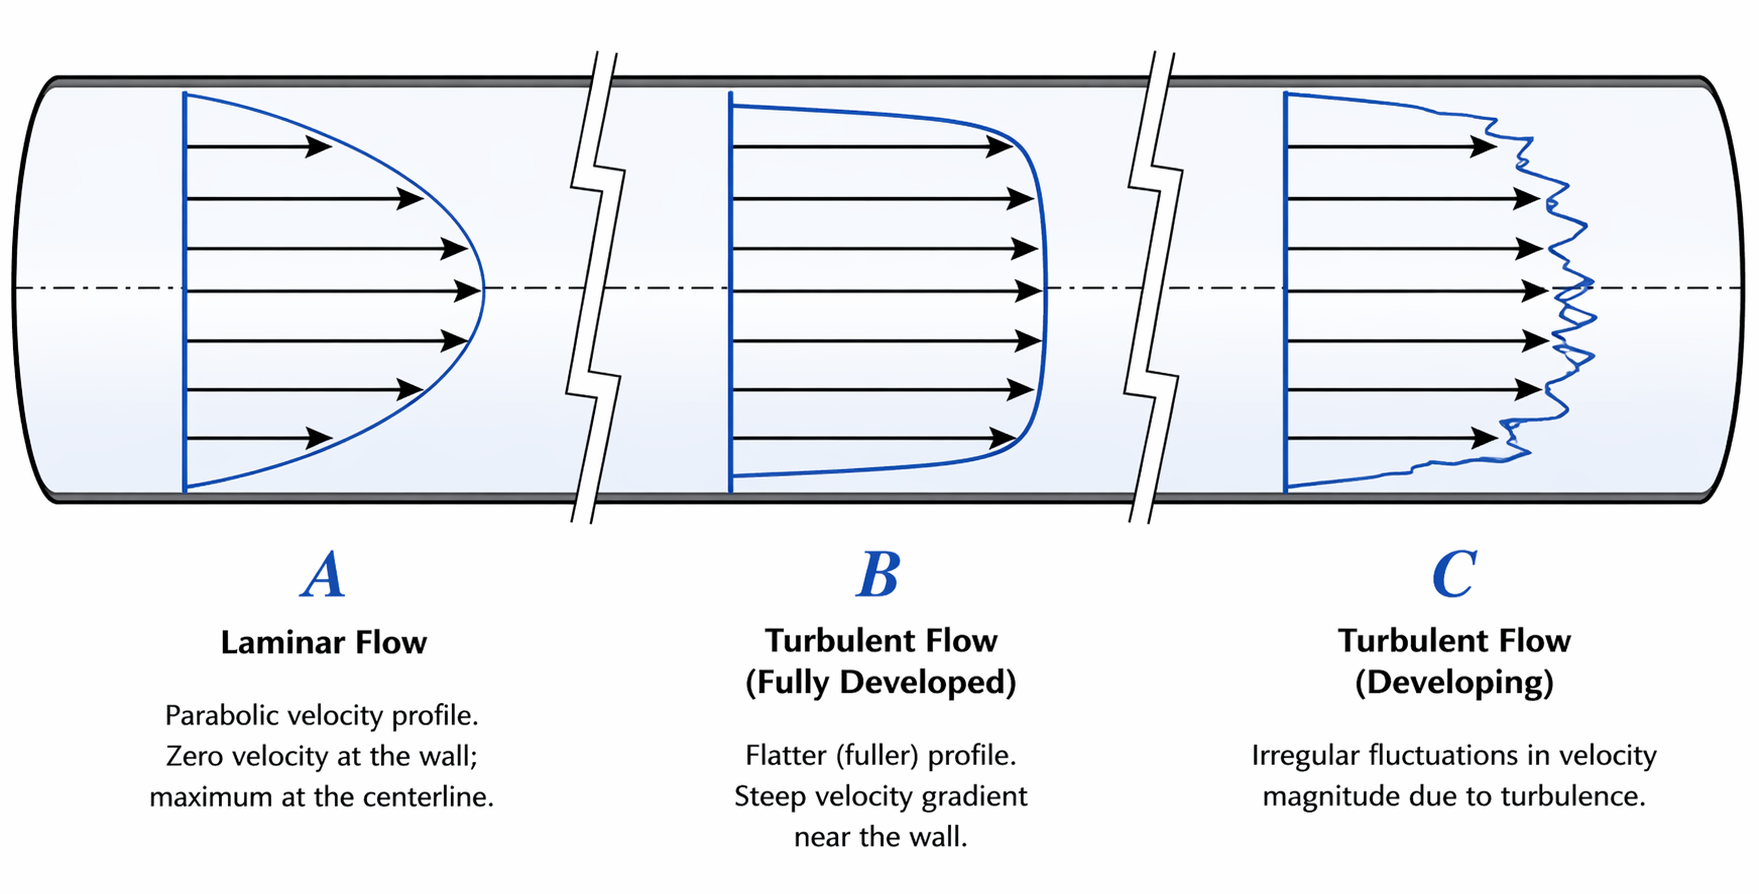
\includegraphics[width=0.82\textwidth]{Lab2_Figures/Vel_profile_updated.png}
    \caption{Velocity profiles for laminar and turbulent pipe flow.}
    \label{fig:velocity-profiles}
\end{figure}

\subsection{Flow Rate, Area, and Continuity}
The mean velocity and volumetric flow rate are related by
\begin{equation}
Q = \bar{V}A
\label{eq:flowrate}
\end{equation}
For a circular pipe,
\begin{equation}
A = \frac{\pi D^2}{4}
\end{equation}
so that
\begin{equation}
\bar{V} = \frac{Q}{A} = \frac{4Q}{\pi D^2}
\label{eq:velocityfromQ}
\end{equation}

Conservation of mass requires
\begin{equation}
Q_1 = Q_2
\qquad \Longrightarrow \qquad
\bar{V}_1 A_1 = \bar{V}_2 A_2
\label{eq:continuity}
\end{equation}
Thus, if the cross-sectional area changes, the average velocity must change inversely.

\subsection{Bernoulli Equation with Head Loss}
The Bernoulli equation between two points along a streamline is
\begin{equation}
\frac{p_1}{\rho g} + \frac{\bar{V}_1^2}{2g} + z_1
=
\frac{p_2}{\rho g} + \frac{\bar{V}_2^2}{2g} + z_2 + h_L
\label{eq:bernoulli-loss}
\end{equation}
where \(h_L\) is the total head loss between points 1 and 2.

The total head loss is split into
\begin{equation}
h_L = h_{L,\text{major}} + h_{L,\text{minor}}
\label{eq:headlosssum}
\end{equation}

\subsubsection*{Important simplification for this lab}
Many segments in this apparatus are horizontal and have constant diameter. In that case,
\[
z_1=z_2
\qquad \text{and} \qquad
\bar{V}_1=\bar{V}_2
\]
so Eq.~\eqref{eq:bernoulli-loss} simplifies to
\begin{equation}
h_L = \frac{p_1-p_2}{\rho g}
\label{eq:horizontal-head-loss}
\end{equation}

This is one of the most important working equations in the lab. It explains why a measured pressure difference across a straight, level, constant-diameter segment can be interpreted directly as a head loss.
\noindent
\textit{Note: The constant-diameter simplification above applies to the
3--2 portion of Figure~\ref{fig:headlosssimple}; the diameter change between
points 2 and 1 requires use of the full energy equation, Eq.~\eqref{eq:bernoulli-loss}.}
\begin{figure}[H]
    \centering
    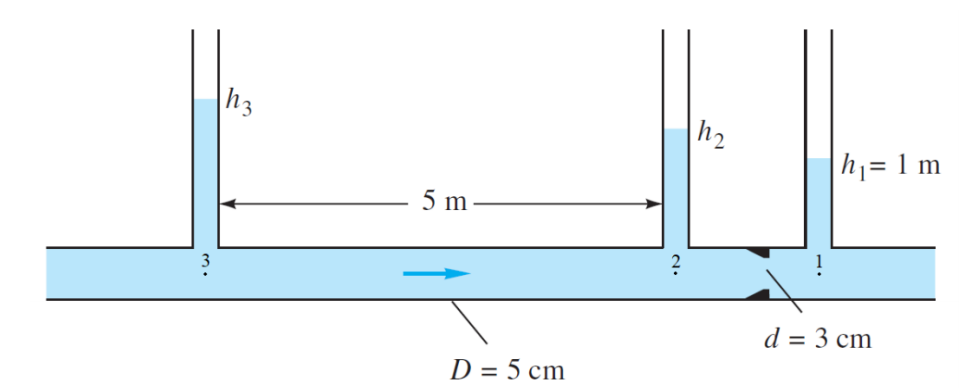
\includegraphics[width=0.82\textwidth]{Lab2_Figures/manometer.png}
    \caption{Depiction of head loss in a simple horizontal pipe section.}
    \label{fig:headlosssimple}
\end{figure}

\subsection{Major Head Loss: Darcy--Weisbach Equation}
For straight-pipe friction over a length \(L\), the major head loss is
\begin{equation}
h_{L,\text{major}} = f\frac{L}{D}\frac{\bar{V}^2}{2g}
\label{eq:darcy}
\end{equation}
where \(f\) is the Darcy friction factor.

\subsubsection*{Laminar flow}
For fully developed laminar flow,
\begin{equation}
f = \frac{64}{Re}
\label{eq:laminarf}
\end{equation}

\subsubsection*{Turbulent flow: implicit and explicit formulas}
For turbulent flow, \(f\) depends on both Reynolds number and relative roughness \(\varepsilon/D\).

The standard implicit relation is the Colebrook--White equation:
\begin{equation}
\frac{1}{\sqrt{f}}
=
-2.0\log_{10}
\left(
\frac{\varepsilon/D}{3.7}
+
\frac{2.51}{Re\sqrt{f}}
\right)
\label{eq:colebrook}
\end{equation}

Because Eq.~\eqref{eq:colebrook} is implicit in \(f\), explicit approximations are often preferred for hand calculations and spreadsheets.

\paragraph{Haaland equation}
A convenient explicit approximation is
\begin{equation}
\frac{1}{\sqrt{f}}
\approx
-1.8\log_{10}
\left[
\left(
\frac{\varepsilon/D}{3.7}
\right)^{1.11}
+
\frac{6.9}{Re}
\right]
\label{eq:haaland}
\end{equation}

\paragraph{Swamee--Jain equation}
Another widely used explicit approximation is
\begin{equation}
f
\approx
0.25
\left[
\log_{10}
\left(
\frac{\varepsilon/D}{3.7}
+
\frac{5.74}{Re^{0.9}}
\right)
\right]^{-2}
\label{eq:swameejain}
\end{equation}

For most turbulent pipe-flow calculations in this course, using Haaland or Swamee--Jain is an efficient alternative to iterating Colebrook or reading directly from the Moody chart.

\subsubsection*{Recommended friction-factor workflow}
For student calculations, the following workflow is recommended:
\begin{enumerate}[leftmargin=*]
    \item Compute \(Q\), \(A\), and \(\bar{V}\).
    \item Compute \(Re\).
    \item If \(Re < 2100\), use Eq.~\eqref{eq:laminarf}.
    \item If \(Re > 4000\), compute \(f\) using Eq.~\eqref{eq:haaland} or Eq.~\eqref{eq:swameejain}.
    \item Optionally cross-check the result against the Moody chart using \(Re\) and \(\varepsilon/D\).
\end{enumerate}

\subsection{Minor Head Loss}
A minor loss due to a fitting is written as
\begin{equation}
h_{L,\text{minor}} = K_L \frac{\bar{V}^2}{2g}
\label{eq:minor}
\end{equation}
where \(K_L\) is the loss coefficient and \(\bar{V}\) is usually the largest relevant mean velocity associated with the fitting.

For this lab, the following correlations are used:

\begin{table}[H]
\centering
\caption{Pipe fittings and their loss-coefficient equations}
\label{tab:KL}
\small
\begingroup
\setlength{\tabcolsep}{4pt}
\begin{tabular}{m{0.17\textwidth} m{0.66\textwidth}}
\toprule
Fitting & Loss coefficient equation \\
\midrule
Elbow at \(90^\circ\) &
ITO equation (turbulent regime):
\[
\begin{aligned}
K_L ={}& 0.367\left(\frac{r}{D}\right)^{-0.84} \\
&+ 1.71\left(\frac{r}{D}\right)^{-1.11}Re^{-0.17}
\end{aligned}
\]
where \(r\) is the radius of curvature of the elbow. \\[1em]

Orifice &
Gibson equation:
\[
K_L = 2.8\left(1-\frac{d}{D}\right)^2
\left[\left(\frac{D}{d}\right)^2 -1\right]
\]
where \(d\) is the orifice diameter. \\[1em]

Sudden expansion &
Carnot equation:
\[
K_L = \left(1-\left(\frac{d}{D}\right)^2\right)^2
\]
where \(d\) is the smaller and \(D\) is the larger diameter. \\[1em]

Sudden contraction &
\[
K_L = 0.42\left(1-\left(\frac{d}{D}\right)^2\right)
\]
where \(d\) is the smaller and \(D\) is the larger diameter. \\
\bottomrule
\end{tabular}
\endgroup
\end{table}

\subsection{How to treat fittings carefully in Bernoulli calculations}
For fittings, do \textbf{not} automatically cancel the kinetic-energy terms. If the diameter changes across the fitting, then \(\bar{V}_1 \neq \bar{V}_2\), and Eq.~\eqref{eq:bernoulli-loss} must be used in full:
\[
\frac{p_1}{\rho g} + \frac{\bar{V}_1^2}{2g} + z_1
=
\frac{p_2}{\rho g} + \frac{\bar{V}_2^2}{2g} + z_2 + h_L
\]
This is especially important for the venturi, orifice, sudden contraction, and sudden expansion.

\subsection{Instrument conversions used in the lab}
Measured pressure differences are often reported in mbar or as manometer height differences. Convert carefully:
\begin{itemize}[leftmargin=*]
    \item DPT reading in mbar \(\rightarrow\) Pa using \(1~\mathrm{mbar}=100~\mathrm{Pa}\)
    \item Pressure difference \(\Delta p\) to head loss using
    \[
    h_L = \frac{\Delta p}{\rho g}
    \]
    \item For water, a manometer reading in mm-H\(_2\)O is already a head difference, so
    \[
    h_L = \Delta h
    \]
    after converting mm to m
\end{itemize}

\subsection{What students should do in each part}
\paragraph{Part 1: Manometer vs DPT}
Use Eq.~\eqref{eq:horizontal-head-loss} to convert both measurements into head loss and compare the instruments directly.

\paragraph{Part 2: Major losses}
Use Eq.~\eqref{eq:darcy} with the appropriate friction factor:
\begin{itemize}[leftmargin=*]
    \item laminar: Eq.~\eqref{eq:laminarf}
    \item turbulent: Eq.~\eqref{eq:haaland} or Eq.~\eqref{eq:swameejain}
\end{itemize}
Then compare theory to measured \(h_L\).

\paragraph{Part 3: Minor losses}
Compute \(K_L\)-based minor losses using Eq.~\eqref{eq:minor}, and include any velocity-head change if the diameter changes.

\paragraph{Part 4: Effect of flow rate}
Since \(\bar{V}\propto Q\), both major and minor losses scale roughly with \(Q^2\) once the friction factor is relatively stable. Thus the measured \(h_L\)-vs-\(Q\) curve should generally be nonlinear and often close to quadratic over the turbulent range.

\section{Procedure}

\subsection*{On Start-Up}
\begin{enumerate}[leftmargin=*]
    \item Ensure that you are wearing all required PPE. Check with your TA that the unit is prepared for the experiment.
    \item Ensure no instrument or other equipment is coupled to any pressure tap before the pump is running.
    \item Ensure at least one line has its valve open, creating an open circuit for flow, at all times.
    \item The main diaphragm valve should be completely shut and then re-opened \(1\) to \(2\) revolutions.
    \item Turn the 3-way valve so that the flow passes through the high-flow flowmeter.
    \item Turn on the pump using the green ON button.
    \item Adjust the main valve to change the flow rate and read the float flowmeter carefully.
    \item Practice taking a flow measurement while reducing parallax error.
    \item Try changing the path of flow by opening a new line valve and then closing the previous one.
\end{enumerate}

Bubbles of air are inevitably introduced when coupling the quick-connect components. Since air differs greatly from water in density and compressibility, trapped bubbles should be purged for each measurement.

\subsection*{Taking Measurements with the Manometer}
\begin{enumerate}[leftmargin=*]
    \item Ensure that the pump is off.
    \item Check that both air-vent valves above and below the left manometer tube are closed.
    \item Carefully attach the quick-couple components of the manometer and pressure taps.
    \item Turn on the pump to flush out air from the pipes.
    \item Place the manometer drain hose in a bucket and open the top air vent valve.
    \item Increase the main flow gradually until the right manometer tube level rises near the top.
    \item Ensure no more bubbles remain, then close the top air vent valve.
    \item Use the manual back-pressure pump \(P_2\) to lower the level in the tubes to half height.
    \item Take the manual reading of the height difference.
    \item Turn off the pump before detaching the quick-connect components.
\end{enumerate}

\subsection*{Taking Measurements with the Differential Pressure Transmitter (DPT)}
\begin{enumerate}[leftmargin=*]
    \item Ensure that the pump is off.
    \item Check that both air-venting valves behind the DPT are closed.
    \item Carefully attach the quick-couple components of the DPT and pressure taps. The DPT red coupling goes upstream and the blue coupling goes downstream.
    \item Turn on the pump to flush out air from the pipes.
    \item Open the air-venting valves behind the DPT to remove trapped bubbles.
    \item Slowly close the air-venting valves after waiting a moment.
    \item Take the pressure-differential reading shown on the screen.
    \item Turn the pump off before detaching the quick-couple components.
\end{enumerate}

\subsection{Part 1: Study of Head Losses using both the Manometer and Differential Pressure Transmitter}
Record pressure-loss measurements using both the manometer and the differential pressure transmitter. Use the high-flow-rate flowmeter and maintain the same flow rate for both measurements. Measure with the manometer first and do not let the flow rate exceed \(4000~\mathrm{L/hr}\) while gradually increasing, unless required for the reading.

\begin{table}[H]
\centering
\caption{Measurements for Part 1}
\label{tab:part1}
\begin{tabular}{ccccc}
\toprule
Pipe & Pipe Segment & Flow Rate, \(Q\) (L/hr) & \(\Delta h_{\text{Manometer}}\) (mm-H\(_2\)O) & \(\Delta P_{\text{DPT}}\) (mbar) \\
\midrule
F & 22--23 & & & \\
\bottomrule
\end{tabular}
\end{table}

\subsection{Part 2: Study of Major Head Losses for Various Pipe Segments}
Record pressure-loss measurements using only the differential pressure transmitter. Use the same flow rate from Part 1.

\begin{table}[H]
\centering
\caption{Measurements for Part 2}
\label{tab:part2}
\begin{tabular}{cccc}
\toprule
Pipe & Pipe Segment & Flow Rate, \(Q\) (L/hr) & \(\Delta P_{\text{DPT}}\) (mbar) \\
\midrule
D & 12--13 & & \\
D & 12--15 & & \\
F & 22--25 & & \\
G & 26--28 & & \\
G & 26--29 & & \\
\bottomrule
\end{tabular}
\end{table}

\subsection{Part 3: Study of Minor Head Losses for Various Pipe Fittings}
Record pressure-loss measurements using only the differential pressure transmitter. Use the same flow rate from Parts 1 and 2.

\begin{table}[H]
\centering
\caption{Measurements for Part 3}
\label{tab:part3}
\begin{tabular}{ccccc}
\toprule
Pipe & Pipe Segment & Fitting & Flow Rate, \(Q\) (L/hr) & \(\Delta P_{\text{DPT}}\) (mbar) \\
\midrule
B & 6--7 & Orifice & & \\
E & 16--17 & Contraction & & \\
E & 18--19 & Expansion & & \\
E & 16--19 & Contraction and expansion & & \\
E & 19--21 & \(90^\circ\) Elbows \(\times 4\) & & \\
\bottomrule
\end{tabular}
\end{table}

\subsection{Part 4: Study of Increasing the Flow Rate for a Pipe Segment}
Choose a pipe segment (excluding elbows) for the analysis. Record pressure-loss measurements using only the differential pressure transmitter for all the flow rates shown.

\begin{table}[H]
\centering
\caption{Measurements for Part 4}
\label{tab:part4}
\begin{tabular}{cccc}
\toprule
Pipe & Pipe Segment & Flow Rate, \(Q\) (L/hr) & \(\Delta P_{\text{DPT}}\) (mbar) \\
\midrule
 & & 500 & \\
 & & 1000 & \\
 & & 2000 & \\
 & & 3000 & \\
 & & 4000 & \\
 & & 5000 & \\
\bottomrule
\end{tabular}
\end{table}

\section{Questions for Analysis}

\subsection*{Part 1}
\begin{enumerate}[leftmargin=*]
    \item Why is there a limit for the flow rate when using the manometer in Part 1? Formulate your answer based on equations from the theoretical background section and the instrument itself.
    \item Compare the total head-loss values you obtained for both devices. You will need to convert mbar to mm-H\(_2\)O. Discuss any differences between both measurements.
    \item Calculate the theoretical head loss for the segment and compare this to your measured values. Discuss sources of error between theoretical and experimental values.
\end{enumerate}

\subsection*{Part 2}
\begin{enumerate}[leftmargin=*]
    \item Compare and discuss the measured values obtained for each segment, including segment 22--23 from Part 1. Formulate your answer based on the characteristics of the pipe segments and the major head-loss equation.
\item Calculate the theoretical major head losses for each segment in pipes F and G and compare these values to your measured values. Use the Darcy--Weisbach equation together with an appropriate friction-factor model: \(f=64/Re\) for laminar flow; identify \(2100 \le Re \le 4000\) as transitional and interpret it with caution; and use Colebrook, Haaland, Swamee--Jain, or the Moody chart for turbulent flow. State which method you used and discuss sources of error between theoretical and experimental values.
    \item Estimate the value for the surface roughness \(\varepsilon\) of pipe D using your measured head-loss values, and compare it to the value used for the smooth pipes. Treat the result as an \emph{effective roughness inferred from the measured head loss}, not as a direct surface measurement.
\end{enumerate}

\subsection*{Part 3}
\begin{enumerate}[leftmargin=*]
    \item Calculate the theoretical minor head losses for each fitting and, if needed, the major head loss for the segments. Compare the total head-loss values to your measured values. Do not forget to consider kinetic-energy changes from Eq.~\eqref{eq:bernoulli-loss}. Discuss sources of error.
    \item Briefly compare the magnitude of the typical minor head-loss values to the typical major head-loss values obtained in Part 2. Do any remarks need to be made about the use of the terms ``minor'' and ``major''?
\end{enumerate}

\subsection*{Part 4}
\begin{enumerate}[leftmargin=*]
\item Plot the measured values of total head loss, \(h_L\), in m, versus the flow rate, \(Q\), in \(\mathrm{m^3/s}\), and add an appropriate trendline that fits the data. Determine the fitted power-law exponent and compare it with the approximate \(h_L \propto Q^2\) behaviour expected when the friction factor is nearly constant. Use the variation of Reynolds number and friction factor with flow rate to explain any systematic departure from an exponent of 2.
\end{enumerate}

\section*{Appendix: Moody Chart Note}
Suppose we are interested in finding a friction factor for a pipe with roughness \(0.04~\mathrm{mm}\), diameter \(2~\mathrm{cm}\), and Reynolds number \(25000\). Since \(Re>4000\), the flow is turbulent. The relative roughness is
\[
\frac{\varepsilon}{D} = \frac{0.04~\mathrm{mm}}{20~\mathrm{mm}} = 0.002.
\]
A vertical line is drawn upward from \(Re=25000\) on the Moody chart until it intersects the relative-roughness line \(\varepsilon/D=0.002\). From that intersection, a horizontal line is drawn to the Darcy friction-factor axis. The chart gives approximately
\[
f \approx 0.029.
\]
Haaland and Swamee--Jain provide explicit turbulent-flow estimates for the same quantity and should give values close to the Moody-chart/Colebrook result for the same \(Re\) and \(\varepsilon/D\).

\begin{figure}[H]
    \centering
    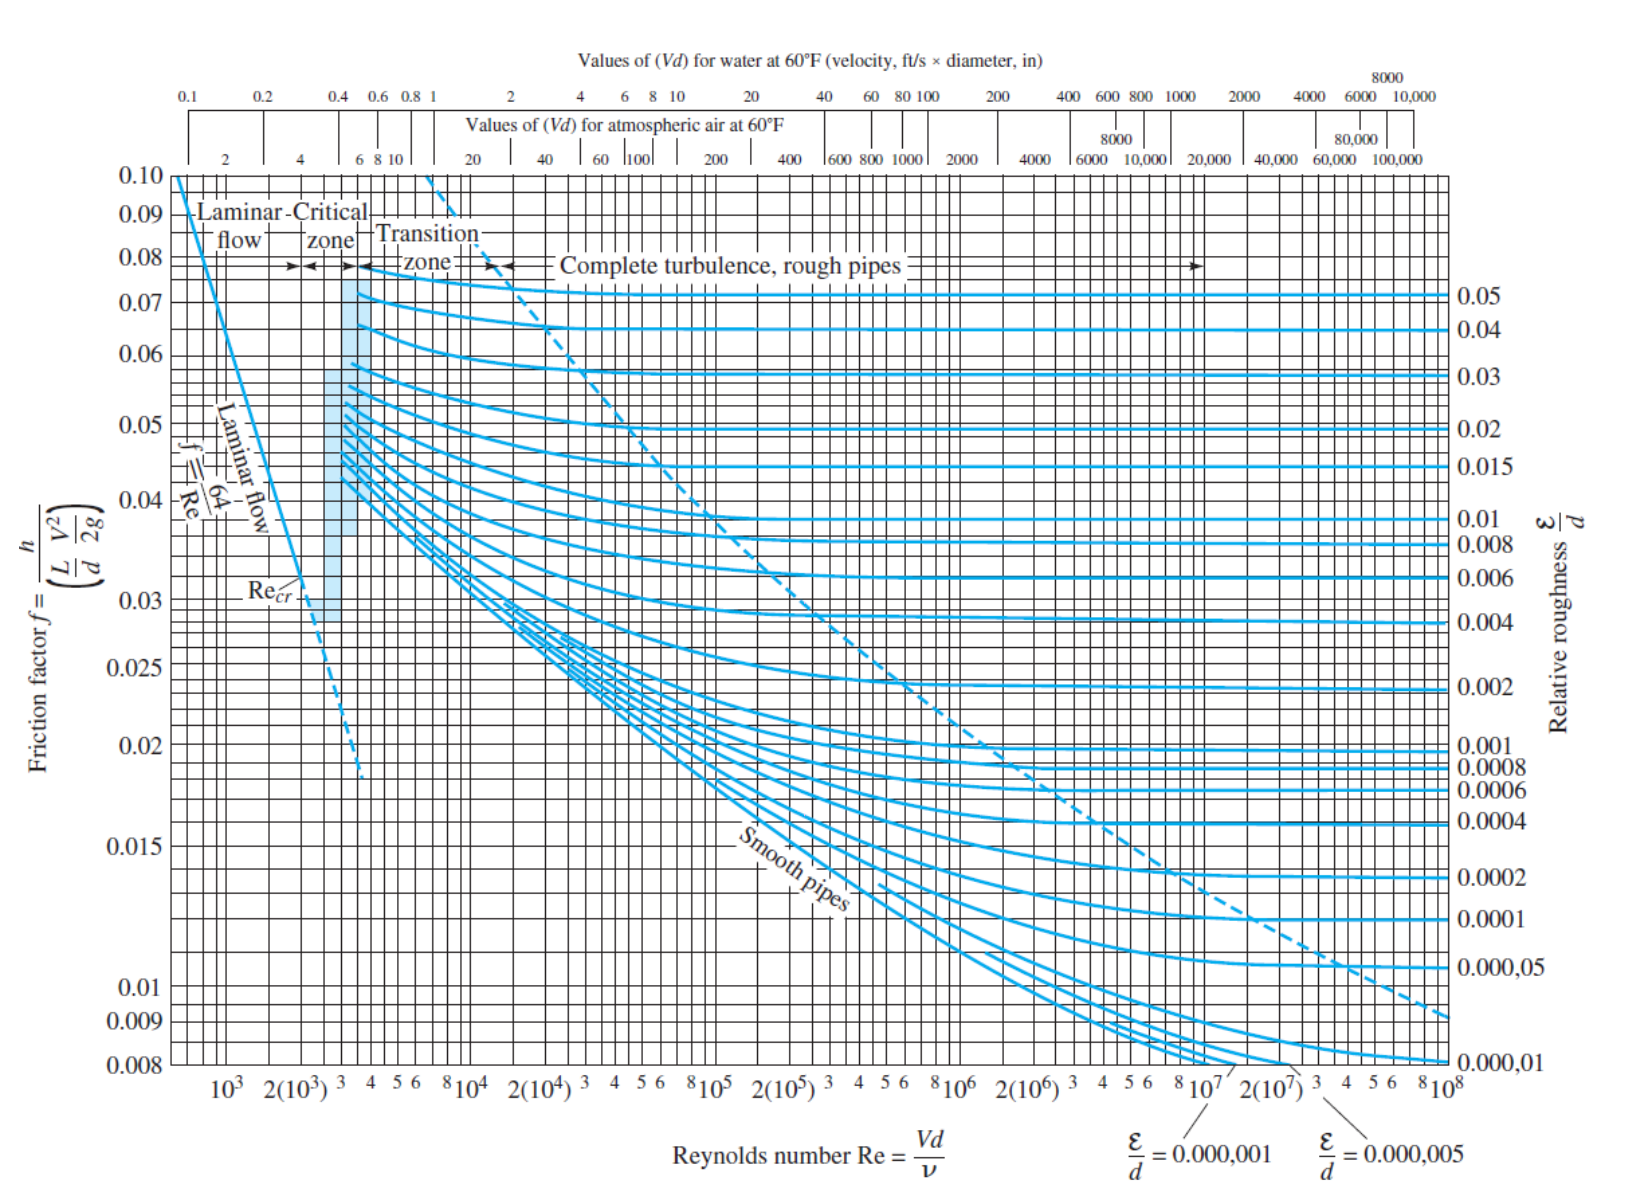
\includegraphics[width=0.98\textwidth]{Lab2_Figures/Moody.png}
    \caption{Moody chart.}
\end{figure}

\section{Recommended Text Readings}

To fully prepare for the experimental and computational components of this lab, students are strongly encouraged to review the relevant sections in the course textbook. The following readings provide the theoretical foundation for the phenomena observed in the laboratory.

\vspace{0.3cm}
\noindent\textbf{Course Textbook Reference:} \\
White, F. M., \& Xue, H. (2020). \textit{Fluid Mechanics} (9th ed.). McGraw-Hill Education. \\
\textit{(*Note: Chapter and section numbering remains consistent with the 8th edition.)}
\vspace{0.3cm}



\subsection*{Lab 2: Internal Flows and Pipe Friction}
\textbf{Primary Focus:} Viscous flow regimes, head loss, friction factors, wall roughness, and minor losses in duct systems.
\begin{itemize}
    \item \textbf{Chapter 6: Viscous Flow in Ducts}
    \begin{itemize}
        \item Section 6.1: Reynolds Number Regimes (Laminar vs. Turbulent transition)
        \item Section 6.3: Head Loss -- The Friction Factor
        \item Section 6.4: Laminar Fully Developed Pipe Flow
        \item Section 6.6: The Moody Chart and Wall Roughness Effects
        \item Section 6.7: Minor or Local Losses in Pipe Systems
    \end{itemize}
    \end{itemize}
\begin{itemize}
        \item Moody, L. F. (1944). "Friction factors for pipe flow." \textit{Transactions of the ASME}, 66(8), 671-684. \url{https://doi.org/10.1115/1.4018140} \textit{(The original publication of the famous Moody chart).}
        \item Fox, R. W., McDonald, A. T., \& Pritchard, P. J. (2020). \textit{Introduction to Fluid Mechanics}. Wiley. \textit{(Provides excellent alternative examples for internal piping networks).}
    \end{itemize}
    





\end{document}
